%% PEng work to date: short report for approval before the full document.
%% Numbers: labbook/2026/catchup*.tex and docs/results.md; PGA and AP rows are the CPU-verified values.
%% Build: latexmk -pdf peng_report.tex
\documentclass[11pt,a4paper]{article}

\usepackage[T1]{fontenc}
\usepackage[utf8]{inputenc}
\usepackage{lmodern}
\usepackage[a4paper,margin=2.2cm]{geometry}
\usepackage{microtype}
\usepackage{amsmath}
\usepackage{array}
\usepackage{booktabs}
\usepackage{float}
\usepackage{xltabular}
\usepackage{xcolor}
\usepackage{caption}
\usepackage{enumitem}
\usepackage{tikz}
\usepackage{pgfplots}
\usepackage[numbers,sort&compress]{natbib}
\usepackage[hidelinks]{hyperref}

\usetikzlibrary{arrows.meta,positioning,calc,fit,backgrounds}
\usepgfplotslibrary{groupplots}
\pgfplotsset{compat=1.18}

\captionsetup{font=normalsize,labelfont=bf,justification=raggedright,singlelinecheck=false}
\captionsetup[table]{skip=4pt}
\setlist{nosep,leftmargin=1.4em,topsep=3pt}
\setlength{\parskip}{5pt}
\setlength{\parindent}{0pt}
\newcolumntype{L}{>{\raggedright\arraybackslash}X}
\newcolumntype{P}[1]{>{\raggedright\arraybackslash}p{#1}}

\newcommand{\Klb}{K_{\mathrm{lb}}}
\definecolor{serieshrnet}{HTML}{2A78D6}
\definecolor{seriesyolo}{HTML}{EB6834}
\definecolor{seriesrtmo}{HTML}{1BAF7A}

\title{PEng Work to Date: Summary for Approval}
\author{Dean Spencer Mills}
\date{}

\begin{document}
\maketitle

\section{Summary}
\label{sec_summary}

The PEng pipeline now groups detected joints to within 0.0004--0.0010 PGA of HigherHRNet's own grouping,
0.0017--0.0027 of YOLO11x-pose's and 0.0064--0.0066 of RTMO-L's, over two training runs.
One trained model serves all three detectors with no retraining.
The MEng pipeline trailed all three by about 0.02 PGA.
The COCO keypoint AP gap fell from 0.099--0.136 to 0.0024--0.0094, but stays above zero on every detector in both runs.

Two ideas produced this.
The first treats grouping as a constrained assignment problem instead of clustering.
The second is a hierarchical PG-GAT, trained on detection-like input, with image evidence along candidate bones.
Six later improvement attempts were tested and none was adopted, so the pipeline has not changed since.
Every number from the final pipeline and its stages was recomputed on the CPU,
and the final recipe was trained twice to measure training noise.

Approval is sought to write the full document on this scope.

\textbf{Terms.}
\begin{itemize}
    \item \textbf{PGA} (pose grouping accuracy): the fraction of joints assigned to the correct person, after aligning
    clusters with annotated people, over detections matched to annotations within 10 px.
    It is scored on one fixed scene set per detector (2,166 HigherHRNet, 2,196 YOLO11x-pose, 2,121 RTMO-L),
    so every row of a table sees identical scenes.
    \item \textbf{AP}: COCO keypoint AP@OKS on all 5,000 val2017 images.
    It scores whole instances, including false positives and missed joints, which PGA does not see.
    \item \textbf{Native}: the detector's own grouping~\citep{cheng2020higherhrnet,ultralytics2024yolo11,lu2024rtmo}.
    \textbf{Gap}: native minus the pipeline being scored, so a negative gap means the pipeline is ahead.
    \item \textbf{Autonomous}: no ground truth at inference.
    \textbf{True K}: the number of annotated people with at least one matched detection, used only as a diagnostic.
    \item \textbf{Intervals}: 95\,\% paired bootstrap over scenes (PGA) or images (AP).
    They do not cover training noise.
\end{itemize}

\section{Assignment rather than clustering}
\label{sec_assignment}

The MEng work treated grouping as clustering: learn a good embedding, then run k-means.
Clustering puts similar points together, and nothing stops it placing two left elbows in one person.
A person is better described as a template with 17 typed slots, each holding at most one joint of that type.
That is an assignment problem, and the PEng work starts from this reformulation.

\textbf{Type constraints on clustering.}
COP-Kmeans~\citep{wagstaff2001copkmeans} adds a cannot-link constraint between joints of the same type.
On a standard GAT and COCO ground-truth keypoints, PGA rose from 0.879 for k-means to 0.910.
Constrained agglomerative (0.887) and spectral (0.894) clustering also beat plain k-means on COCO.

\textbf{Optimal transport (SCOT).}
SCOT defines $K \times 17$ typed slots with learned person prototypes, infinite cost on a type mismatch and
Sinkhorn~\citep{cuturi2013sinkhorn} iterations.
It reached 0.923 on synthetic data but 0.862 on COCO, below COP-Kmeans.
Four variants stayed at 0.83--0.87 and other training strategies at 0.86--0.88.
SCOT-KI replaced the prototypes with k-means centroids of the scene and recovered 6.5 points, reaching 0.926.
It stayed 4.2 points below COP-Kmeans on the same embedding, which isolates the Sinkhorn step as the fault.
The ranking held on HigherHRNet backbone features too, so the embedding is not the cause.

\textbf{Type-wise Hungarian assignment (THA).}
THA replaces Sinkhorn with one optimal matching per joint type.
Starting from k-means centroids $\mu_k$, the $M_t$ joints of each type $t$ are matched one-to-one to the $K$ centroids,
\begin{equation}
    \pi_t^\ast = \operatorname*{arg\,min}_{\pi_t} \sum_{j\,:\,\mathrm{type}(j)=t} \left\| e_j - \mu_{\pi_t(j)} \right\|_2 ,
    \label{eq:tha}
\end{equation}
by the Hungarian algorithm~\citep{kuhn1955hungarian}, where $e_j$ is the embedding of joint $j$.
Centroids are then recomputed from the joints of all types, and the steps repeat for up to 10 iterations.
Two joints of one type cannot share a person by construction, and the method has no learned parameters.
No prior method with this decomposition was found:
OpenPose~\citep{cao2017openpose} matches pairs of adjacent types instead of one type against person centroids.
Table~\ref{tab:methods} compares these methods on one embedding.

\begin{table}[H]
\centering
\caption{Grouping methods on one embedding (COCO-fine-tuned SA-GAT, true K), PGA. Detections are HigherHRNet's.}
\label{tab:methods}
\begin{tabular}{lccc}
\toprule
Method & Synthetic & COCO GT keypoints & Detections \\
\midrule
k-means & 0.928 & 0.957 & 0.942 \\
SCOT, fixed prototypes & 0.838 & 0.861 & --- \\
SCOT-KI & --- & 0.926 & --- \\
COP-Kmeans & 0.938 & 0.968 & 0.955 \\
\textbf{THA} & \textbf{0.965} & \textbf{0.969} & \textbf{0.955} \\
\bottomrule
\end{tabular}
\end{table}

\textbf{A feasibility bound on K.}
A type-constrained grouping with fewer clusters than the most frequent joint type must violate the constraint.
The pipeline therefore never lets K fall below that count:
\begin{equation}
    \Klb = \max_t M_t , \qquad K = \max\bigl(\hat{K}, \Klb\bigr) ,
    \label{eq:clamp}
\end{equation}
where $\hat{K}$ is the K-head prediction.
The rule adds no parameters.
Table~\ref{tab:krule} shows the effect of K rule and grouping method on the unchanged MEng embedding.

\begin{table}[H]
\centering
\caption{K rule and grouping method on the MEng embedding, 2,166 HigherHRNet scenes (native 0.9849), PGA.}
\label{tab:krule}
\begin{tabular}{lccccc}
\toprule
K rule & Mean K & k-means & COP-Kmeans & THA & Gap (best) \\
\midrule
Annotated people (MEng protocol) & 2.74 & 0.9588 & 0.9634 & 0.9631 & 0.0215 \\
K-head alone (MEng autonomous) & 2.46 & 0.9644 & 0.9657 & 0.9660 & 0.0189 \\
$\Klb$ alone & 2.46 & 0.9714 & 0.9753 & 0.9757 & 0.0093 \\
\textbf{Clamp, Equation~\eqref{eq:clamp}} & \textbf{2.55} & \textbf{0.9715} & \textbf{0.9752} & \textbf{0.9755} & \textbf{0.0094} \\
True K (diagnostic) & 2.59 & 0.9750 & 0.9798 & 0.9797 & 0.0052 \\
\bottomrule
\end{tabular}
\end{table}

With no change to the embedding, the autonomous gap fell from 0.0205 to 0.0094 [0.0070, 0.0119].
The K rule contributed about 0.0070 and constrained assignment about 0.0041.
In AP, THA with $\Klb$ added 0.0805 / 0.1101 / 0.0847 over the MEng pipeline on the three detectors,
the largest single step of the work.

\textbf{THA and COP-Kmeans cannot be separated on real data.}
Under the clamp the difference is +0.0004 [$-$0.0004, +0.0011], and both reach 0.955 on detections in
Table~\ref{tab:methods}.
THA's clear lead is on synthetic data (0.965 against 0.938), and it needs no restarts:
10 restarts gave +0.0000 on synthetic data and $-$0.0002 on COCO, while COP-Kmeans uses 10.
The evidence supports constrained assignment over clustering, not THA over COP-Kmeans on COCO.

\section{PG-GAT updates}
\label{sec_pggat}

Table~\ref{tab:krule} leaves a gap of 0.0052 at true K, so the embedding had to improve as well.
That gap is genuine: PG-GAT beats native on the joints HigherHRNet's refine step adds (0.926 against 0.895),
and trails it on ordinary heatmap peaks (0.975 against 0.985).
Figure~\ref{fig:pipeline} shows the resulting pipeline and Table~\ref{tab:updates} the five changes.

\begin{figure}[H]
\centering
\resizebox{\linewidth}{!}{%
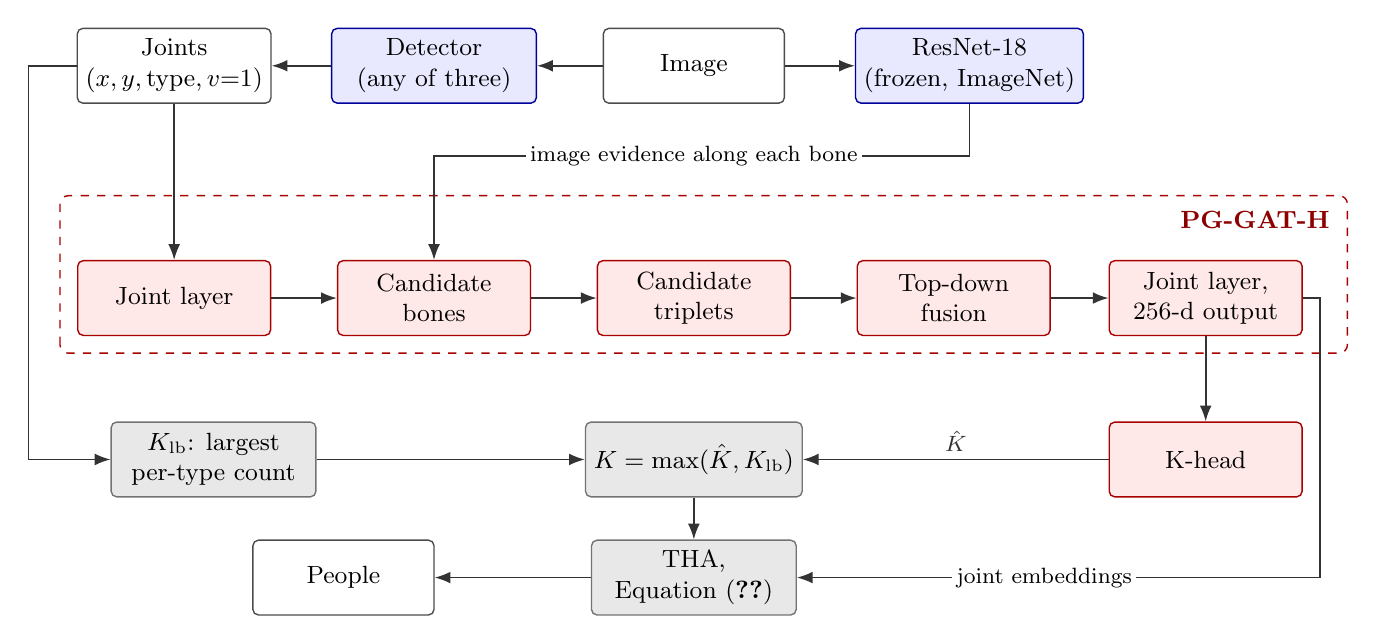
\begin{tikzpicture}[
    >={Latex[length=2mm]},
    every node/.style={font=\small,align=center},
    box/.style={draw,rounded corners=2pt,minimum height=0.95cm,inner sep=3pt,line width=0.5pt},
    data/.style={box,draw=black!70,fill=white,minimum width=2.3cm},
    ext/.style={box,draw=blue!60!black,fill=blue!9,minimum width=2.6cm},
    trained/.style={box,draw=red!65!black,fill=red!9,minimum width=2.45cm},
    det/.style={box,draw=black!55,fill=black!9,minimum width=2.6cm},
    flow/.style={->,line width=0.6pt,black!80},
    lab/.style={font=\footnotesize,fill=white,inner sep=1.5pt}
]
% row 1: inputs
\node[data] (joints) at (1.45,0) {Joints\\$(x, y, \mathrm{type}, v{=}1)$};
\node[ext] (det) at (4.75,0) {Detector\\(any of three)};
\node[data] (img) at (8.05,0) {Image};
\node[ext] (res) at (11.55,0) {ResNet-18\\(frozen, ImageNet)};
\draw[flow] (img) -- (det);
\draw[flow] (det) -- (joints);
\draw[flow] (img) -- (res);

% row 2: PG-GAT-H
\node[trained] (j1) at (1.45,-2.95) {Joint layer};
\node[trained] (bones) at (4.75,-2.95) {Candidate\\bones};
\node[trained] (trip) at (8.05,-2.95) {Candidate\\triplets};
\node[trained] (fus) at (11.35,-2.95) {Top-down\\fusion};
\node[trained] (j2) at (14.55,-2.95) {Joint layer,\\256-d output};
\begin{scope}[on background layer]
    \draw[red!65!black,dashed,rounded corners=3pt,line width=0.5pt] (0,-3.65) rectangle (16.35,-1.65);
\end{scope}
\node[font=\small\bfseries,text=red!55!black,anchor=north east] at (16.25,-1.72) {PG-GAT-H};
\draw[flow] (joints) -- (j1);
\draw[flow] (j1) -- (bones);
\draw[flow] (bones) -- (trip);
\draw[flow] (trip) -- (fus);
\draw[flow] (fus) -- (j2);
\draw[flow] (res.south) -- (11.55,-1.15) -- (4.75,-1.15) -- (bones.north);
\node[lab] at (8.05,-1.15) {image evidence along each bone};

% row 3: K
\node[det] (klb) at (1.95,-5.0) {$\Klb$: largest\\per-type count};
\node[det] (clamp) at (8.05,-5.0) {$K = \max(\hat{K}, \Klb)$};
\node[trained] (khead) at (14.55,-5.0) {K-head};
\draw[flow] (j2) -- (khead);
\draw[flow] (khead) -- node[lab,above=1pt] {$\hat{K}$} (clamp);
\draw[flow] (klb) -- (clamp);
\draw[flow] (joints.west) -- (-0.4,0) -- (-0.4,-5.0) -- (klb.west);

% row 4: assignment
\node[det] (tha) at (8.05,-6.5) {THA,\\Equation~\eqref{eq:tha}};
\node[data] (people) at (3.6,-6.5) {People};
\draw[flow] (clamp) -- (tha);
\draw[flow] (tha) -- (people);
\draw[flow] (j2.east) -- (16.0,-2.95) -- (16.0,-6.5) -- (tha.east);
\node[lab] at (12.5,-6.5) {joint embeddings};
\end{tikzpicture}%
}
\caption{The PEng pipeline. The detector is HigherHRNet, YOLO11x-pose or RTMO-L.
Red: trained in this work. Blue: external or frozen. Grey: deterministic, no parameters.}
\label{fig:pipeline}
\end{figure}

\begin{table}[H]
\centering
\caption{The five updates. PGA on HigherHRNet scenes against the previous step unless stated;
three values are HigherHRNet / YOLO11x-pose / RTMO-L.}
\label{tab:updates}
\begin{tabularx}{\linewidth}{@{}P{2.3cm}LL@{}}
\toprule
Update & What changed & Effect on detections \\
\midrule
Hierarchy (PG-GAT-H)
& Joints, candidate bones (3 nearest detections per adjacent type), candidate triplets,
then validity-weighted fusion back into joints.
No person labels and no voting.
& Alone: $-$0.0017 [$-$0.0034, +0.0001], despite +0.0098 on COCO GT keypoints.
Dropping 20\,\% of joints removes its advantage. \\
\addlinespace
Detection-like training
& Joint dropout $p \sim U(0, 0.4)$ per training graph, visibility fixed at 1.
& $\Klb$ THA +0.0019 [+0.0004, +0.0034], true K +0.0031 [+0.0013, +0.0049].
Flat control: $-$0.0004, so the gain is the hierarchy's. \\
\addlinespace
Image evidence
& Frozen ImageNet ResNet-18 (stride 16), 5 samples along each candidate bone, zero-initialised branch.
& $\Klb$ THA +0.0018 [+0.0008, +0.0029], true K +0.0025 [+0.0012, +0.0038].
True-K gain +0.0021 to +0.0026 on all three. \\
\addlinespace
Augmented K-head
& K-head on frozen embeddings with the same dropout, selected on held-out COCO train images.
& Clamp minus $\Klb$ THA: +0.0034 / +0.0038 / +0.0028, intervals above zero.
Control on the MEng embedding: $-$0.0037. \\
\addlinespace
Crowd over-sampling (3$\times$)
& Images with 6 or more people go from 12.1\,\% to 29.2\,\% of samples, with epoch size unchanged.
& Two runs per arm, 6 or more people: +0.0040 / +0.0041 / +0.0030.
All scenes: +0.0012 / +0.0009 / +0.0005. \\
\bottomrule
\end{tabularx}
\end{table}

\textbf{Cost.}
The grouping pipeline has 3.30M parameters: 479,794 trainable in PG-GAT-H, 35,009 in the K-head and 2,782,784 frozen in
the backbone.
THA and the clamp add none.
These sit on top of the detector,
whereas HigherHRNet's own tag head has about 561 parameters~\citep{newell2017associative}.
The pipeline is therefore much larger than the grouping it replaces.
What it gains is that one model works on any detector without retraining.

\section{Results}
\label{sec_results}

Table~\ref{tab:stages} and Figure~\ref{fig:stages} show the gap after each cumulative stage, one training run per row.
The gap falls at every stage, on every detector and in both metrics.
The smallest steps are comparable to training noise: stage E overall, and stage D for HigherHRNet AP.

\begin{table}[H]
\centering
\caption{Gap to native after each stage. PGA rows B--E use clamp THA; AP rows B--E use $\Klb$ THA with every detected
joint (threshold 0). HRNet is HigherHRNet.}
\label{tab:stages}
\begin{tabular}{@{}llcccccc@{}}
\toprule
& & \multicolumn{3}{c}{PGA gap} & \multicolumn{3}{c}{AP gap} \\
\cmidrule(lr){3-5} \cmidrule(l){6-8}
& Stage & HRNet & YOLO & RTMO & HRNet & YOLO & RTMO \\
\midrule
A & MEng: K-head, k-means & 0.0205 & 0.0210 & 0.0220 & 0.1177 & 0.1360 & 0.0994 \\
B & + THA, K bound & 0.0094 & 0.0103 & 0.0141 & 0.0371 & 0.0259 & 0.0147 \\
C & + hierarchy, training, K-head & 0.0061 & 0.0063 & 0.0102 & 0.0144 & 0.0102 & 0.0062 \\
D & + image evidence & 0.0017 & 0.0034 & 0.0069 & 0.0116 & 0.0056 & 0.0036 \\
\textbf{E} & \textbf{+ crowd over-sampling} & \textbf{0.0004} & \textbf{0.0017} & \textbf{0.0064} & \textbf{0.0076} & \textbf{0.0050} & \textbf{0.0024} \\
\bottomrule
\end{tabular}
\end{table}

\begin{figure}[H]
\centering
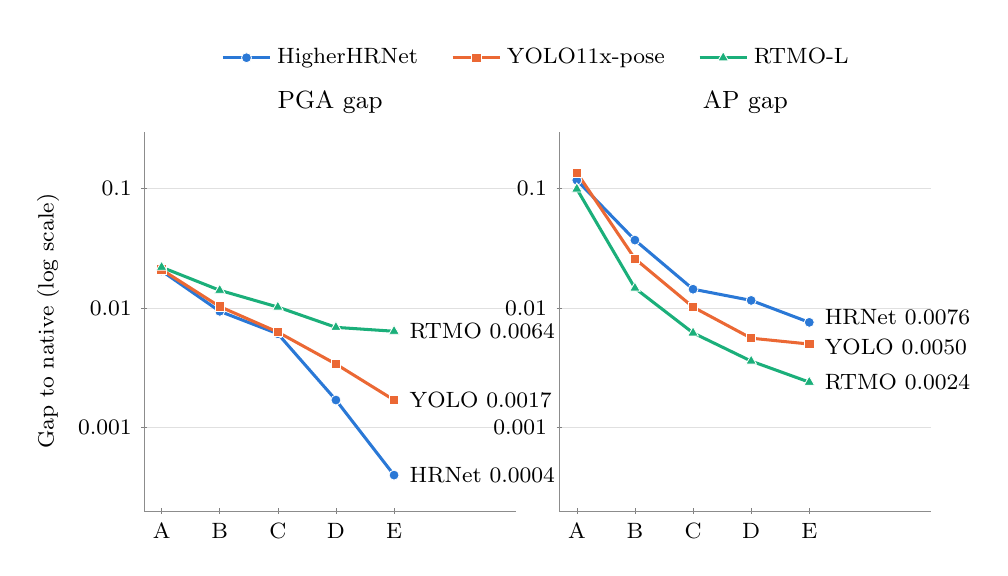
\begin{tikzpicture}
\pgfplotsset{
    gap/.style={
        width=0.52\linewidth, height=6.4cm,
        ymode=log, ymin=2e-4, ymax=0.3,
        xmin=0.7, xmax=7.1,
        xtick={1,2,3,4,5}, xticklabels={A,B,C,D,E},
        ytick={0.001,0.01,0.1}, yticklabels={0.001,0.01,0.1},
        minor y tick style={draw=none}, major tick length=2pt,
        axis lines=left, axis line style={black!45,-},
        ymajorgrids, major grid style={black!12},
        tick label style={font=\footnotesize}, label style={font=\footnotesize},
        title style={font=\small,yshift=-3pt},
        clip=false,
    },
    hr/.style={serieshrnet,line width=1.1pt,mark=*,mark size=1.8pt,mark options={fill=serieshrnet,draw=white,line width=0.3pt}},
    yo/.style={seriesyolo,line width=1.1pt,mark=square*,mark size=1.7pt,mark options={fill=seriesyolo,draw=white,line width=0.3pt}},
    rt/.style={seriesrtmo,line width=1.1pt,mark=triangle*,mark size=2.2pt,mark options={fill=seriesrtmo,draw=white,line width=0.3pt}},
}
\begin{groupplot}[group style={group size=2 by 1,horizontal sep=0.55cm},gap]
\nextgroupplot[title={PGA gap},ylabel={Gap to native (log scale)},
    legend to name=stagelegend,legend columns=3,
    legend style={draw=none,font=\footnotesize,/tikz/every even column/.append style={column sep=10pt}}]
\addplot[hr] coordinates {(1,0.0205)(2,0.0094)(3,0.0061)(4,0.0017)(5,0.0004)};
\addlegendentry{HigherHRNet}
\addplot[yo] coordinates {(1,0.0210)(2,0.0103)(3,0.0063)(4,0.0034)(5,0.0017)};
\addlegendentry{YOLO11x-pose}
\addplot[rt] coordinates {(1,0.0220)(2,0.0141)(3,0.0102)(4,0.0069)(5,0.0064)};
\addlegendentry{RTMO-L}
\node[anchor=west,font=\footnotesize] at (axis cs:5.1,0.0064) {RTMO 0.0064};
\node[anchor=west,font=\footnotesize] at (axis cs:5.1,0.0017) {YOLO 0.0017};
\node[anchor=west,font=\footnotesize] at (axis cs:5.1,0.0004) {HRNet 0.0004};
\nextgroupplot[title={AP gap}]
\addplot[hr] coordinates {(1,0.1177)(2,0.0371)(3,0.0144)(4,0.0116)(5,0.0076)};
\addplot[yo] coordinates {(1,0.1360)(2,0.0259)(3,0.0102)(4,0.0056)(5,0.0050)};
\addplot[rt] coordinates {(1,0.0994)(2,0.0147)(3,0.0062)(4,0.0036)(5,0.0024)};
\node[anchor=west,font=\footnotesize] at (axis cs:5.1,0.0084) {HRNet 0.0076};
\node[anchor=west,font=\footnotesize] at (axis cs:5.1,0.0047) {YOLO 0.0050};
\node[anchor=west,font=\footnotesize] at (axis cs:5.1,0.0024) {RTMO 0.0024};
\end{groupplot}
\node[anchor=south] at ($(group c1r1.north)!0.5!(group c2r1.north)+(0,0.55)$) {\pgfplotslegendfromname{stagelegend}};
\end{tikzpicture}
\caption{Gap to native after stages A--E of Table~\ref{tab:stages}, on one shared log scale.}
\label{fig:stages}
\end{figure}

The final recipe was trained twice.
The first run turned out to be the better one, so its numbers in Table~\ref{tab:stages} are optimistic by about one
noise draw.
Tables~\ref{tab:pga} and~\ref{tab:ap} give both runs.

\begin{table}[H]
\centering
\caption{Final recipe, PGA with THA, two training runs.}
\label{tab:pga}
\begin{tabular}{@{}lccc@{}}
\toprule
& HigherHRNet & YOLO11x-pose & RTMO-L \\
\midrule
Native & 0.9849 & 0.9863 & 0.9961 \\
Autonomous, run 1 / run 2 & 0.9845 / 0.9840 & 0.9846 / 0.9837 & 0.9897 / 0.9895 \\
\addlinespace
Autonomous gap, run 1 & 0.0004 & 0.0017 & 0.0064 \\
& [$-$0.0016, 0.0025] & [$-$0.0007, 0.0042] & [0.0051, 0.0078] \\
Autonomous gap, run 2 & 0.0010 & 0.0027 & 0.0066 \\
& [$-$0.0012, 0.0031] & [0.0001, 0.0053] & [0.0053, 0.0080] \\
\addlinespace
True-K gap, run 1 & $-$0.0024 & $-$0.0005 & 0.0062 \\
& [$-$0.0043, $-$0.0005] & [$-$0.0028, 0.0017] & [0.0048, 0.0077] \\
True-K gap, run 2 & $-$0.0005 & 0.0002 & 0.0059 \\
& [$-$0.0027, 0.0016] & [$-$0.0022, 0.0025] & [0.0046, 0.0073] \\
\bottomrule
\end{tabular}
\end{table}

\begin{table}[H]
\centering
\caption{Final recipe, AP with $\Klb$ THA at threshold 0, two training runs. Intervals are BCa.
On RTMO-L run 2 the BCa interval is unstable; its percentile interval is [0.0004, 0.0040].}
\label{tab:ap}
\begin{tabular}{@{}lccc@{}}
\toprule
& HigherHRNet & YOLO11x-pose & RTMO-L \\
\midrule
Native & 0.5834 & 0.6666 & 0.6460 \\
Pipeline, run 1 / run 2 & 0.5758 / 0.5740 & 0.6616 / 0.6613 & 0.6436 / 0.6426 \\
\addlinespace
Gap, run 1 & 0.0076 & 0.0050 & 0.0024 \\
& [0.0035, 0.0100] & [0.0027, 0.0082] & [0.0018, 0.0049] \\
Gap, run 2 & 0.0094 & 0.0053 & 0.0034 \\
& [0.0064, 0.0130] & [0.0030, 0.0083] & [0.0030, 0.0068] \\
\addlinespace
K-head clamp row, gap, run 1 & 0.0182 & 0.0225 & 0.0208 \\
& [0.0132, 0.0208] & [0.0185, 0.0249] & [0.0176, 0.0251] \\
\addlinespace
AP with perfect grouping (estimate) & 0.627 & 0.678 & 0.646 \\
\bottomrule
\end{tabular}
\end{table}

\textbf{Where the AP gap comes from.}
It is single wrong joints in people who are found, mostly in crowds, and not missed people or ranking.
At OKS 0.50 the pipeline is level with or ahead of native on all three detectors.
Giving its instances the native scores recovers nothing.
It loses 528 / 164 / 50 correct joint slots and wins 181 / 27 / 1.
Of the people who fall below OKS 0.75, about 70\,\% are in scenes with 6 or more people,
and about 40--45\,\% differ from native in one joint.
In about 70\,\% of lost slots the joint native kept is the more confident one, and the model never sees confidence.

\textbf{What the evidence supports.}
\begin{itemize}
    \item Constrained assignment and the K bound improve on clustering by a wide margin on the same embedding.
    \item PGA parity with HigherHRNet holds in both runs.
    YOLO11x-pose is within 0.002--0.003: its interval includes zero in one run of two, so parity is not claimed.
    \item RTMO-L keeps a real gap of about 0.006 PGA even at true K.
    \item The AP gap is above zero on all three detectors in both runs, under both interval methods.
    \item Crowd over-sampling is a replicated gain of 0.003--0.004 PGA in scenes with 6 or more people, and at most
    0.0013 overall.
    Doubling it to 6$\times$ adds nothing measurable.
\end{itemize}

\textbf{Limits of these claims.}
\begin{itemize}
    \item \textbf{Training noise.} Two runs of one recipe differ by about 0.001 PGA overall.
    On HigherHRNet AP they differ by up to 0.004: four runs of 3$\times$ and 6$\times$ give gaps of 0.0055--0.0096.
    Scene and image intervals do not cover this, so a gap should be quoted as a range over runs.
    \item \textbf{Being ahead at true K.} The lead over HigherHRNet holds for run 1 only and is not claimed.
    \item \textbf{K rule differs by metric.} The AP row uses $\Klb$, which at threshold 0 equals the detector's own
    instance count.
    It uses no ground truth, but it borrows the detector's person count and re-shuffles the detector's joints.
    Adding the K-head (the PGA rule) raises the AP gap to about 0.02, because the head over-counts on the
    false-positive-heavy pool.
    \item \textbf{No untouched test set.} All numbers are on val2017, the same images that guided the design decisions.
    \item \textbf{``No retraining'' is about training only.} No model was trained on any detector's output,
    but the YOLO11x-pose and RTMO-L rows did guide later choices, such as crowd over-sampling.
    \item \textbf{Early numbers.} The early assignment results (Table~\ref{tab:methods}) stand as recorded at
    the time and were not part of the verification.
    The lab book also holds two sets of SCOT variant numbers; the range quoted covers both, and the conclusion is the
    same under either.
    \item \textbf{Runtime.} Inference time of the pipeline has not been measured.
    \item \textbf{Single runs remain.} The hierarchy's attribution rests on one run each of PG-GAT-H + training and the
    flat control.
    The K-head of record was the best of several, so its K-head AP rows are optimistic.
\end{itemize}

\section{All experiments}
\label{sec_experiments}

Table~\ref{tab:experiments} lists the PEng experiments by phase, as recorded in the lab book.
Three values are HigherHRNet / YOLO11x-pose / RTMO-L, and $\Delta$ is the new arm minus the baseline.
``Autonomous'' is clamp THA.

\begin{xltabular}{\linewidth}{@{}P{4.2cm}LP{2.15cm}@{}}
\caption{Every PEng experiment, its result and the decision taken.}
\label{tab:experiments} \\
\toprule
Experiment & Result & Decision \\
\midrule
\endfirsthead
\toprule
Experiment & Result & Decision \\
\midrule
\endhead
\bottomrule
\endlastfoot
\multicolumn{3}{@{}l}{\textbf{Assignment methods} (COCO GT keypoints, true K)} \\
Type constraints on clustering & k-means 0.879; COP-Kmeans 0.910, spectral 0.894, agglomerative 0.887 & Kept \\
SCOT (typed optimal transport) & Synthetic 0.923, COCO 0.862 & Not adopted \\
SCOT variants: residual, adaptive, unbalanced, dustbin & COCO 0.83--0.87, none above COP-Kmeans & Not adopted \\
SCOT training: joint COCO fine-tune, frozen GAT, standard GAT & COCO 0.884, 0.861, 0.881 & Not adopted \\
SCOT-KI (k-means prototypes) & 0.926, against COP-Kmeans 0.968 on one embedding: Sinkhorn is the fault & Not adopted \\
Methods on HigherHRNet backbone features & k-means 0.789, COP-Kmeans 0.891, THA 0.884, SCOT-KI 0.825: same ranking, so not the embedding & Diagnostic \\
THA & Synthetic 0.965, COCO 0.969, detections 0.955 & Adopted \\
K-head training & Frozen on COCO: exact K 79.6\,\%, COP-Kmeans 0.950. Joint: 55.5\,\%, 0.677, though a later re-run lost only 0.015 PGA & Frozen kept \\
Autonomous SCOT pipeline & Detections, K-head: SCOT 0.800, COP-Kmeans 0.816 & Not adopted \\
\addlinespace
\multicolumn{3}{@{}l}{\textbf{Test-time compute} (MEng embedding)} \\
THA with 10 restarts & +0.0000 synthetic, $-$0.0002 COCO GT & Not adopted \\
K selection by silhouette & K exact 39--46\,\%, costs about 0.15 PGA & Not adopted \\
K feasibility clamp & Detections 0.9644 to 0.9755 & Adopted \\
\addlinespace
\multicolumn{3}{@{}l}{\textbf{Pipeline}} \\
Fixed-scene gap table & Gap 0.0094 [0.0070, 0.0119]: K 0.0042, embedding 0.0052; $\Klb$ alone ties the clamp & Benchmark \\
HigherHRNet without refine & Same peaks: PG-GAT 0.9745, tag matching 0.8666; AP falls 0.492 to 0.386, so refine also detects. Final pipeline on these peaks: 0.9823 & Diagnostic \\
PG-GAT-H, first run & COCO GT THA +0.0098, detections $-$0.0017 & Kept \\
Shift diagnostic & Dropping 20\,\% of joints removes the advantage; jitter costs nothing & Diagnostic \\
Detection-like training with flat control & $\Klb$ THA +0.0019 with hierarchy, $-$0.0004 flat & Adopted \\
Gap by joint origin & Deficit is on heatmap peaks (0.985 against 0.975), so the missing information is in the image & Diagnostic \\
K from bone validity & THA 0.8465 to 0.9722, against $\Klb$ 0.9755; pieces 1.6--9\,\% impure & Not adopted \\
Coordinate frame check & Letterbox frame $-$0.0007 [$-$0.0015, +0.0001] & Immaterial \\
Image evidence along bones & $\Klb$ THA +0.0018, true K +0.0025 & Adopted \\
Augmented K-head & Clamp minus $\Klb$ THA +0.0034 / +0.0038 / +0.0028 & Adopted \\
Detector swap (no retraining) & $\Klb$ THA over stage B +0.0041 / +0.0031 / +0.0044 & Evaluation \\
AP@OKS on three detectors & Threshold 0 with $\Klb$ THA is the best AP rule & Evaluation \\
Crowd over-sampling, 3$\times$ & Autonomous +0.0013 / +0.0017 / +0.0005, one run & Adopted \\
\addlinespace
\multicolumn{3}{@{}l}{\textbf{Verification and noise}} \\
Verification of every number & 2,282 metrics on the CPU; largest change 0.0007 PGA, 0.0024 AP; no conclusion changes & CPU values canonical \\
Diagnostics & With K right, error 0.79\,\% / 0.74\,\% / 0.48\,\% against native 1.67\,\% / 0.99\,\% / 0.06\,\%; weak on large people and in crowds & Diagnostic \\
AP confidence intervals & AP gap above zero on all three; BCa and percentile both required & Method kept \\
Fine-tune seed repeat & Noise about 0.001 PGA; 3 of 12 same-recipe intervals exclude zero & Two runs per arm \\
No-crowd repeat ($2 \times 2$ runs) & 6+ people +0.0040 / +0.0041 / +0.0030; AP in 6+ images +0.0051 / +0.0035 / +0.0007 & 3$\times$ kept \\
\addlinespace
\multicolumn{3}{@{}l}{\textbf{Improvement attempts on the final pipeline}} \\
K-head with per-type count histogram & Autonomous $-$0.0006 / $-$0.0011 / $-$0.0009, despite better held-out K (0.912 against 0.899) & Not adopted \\
Same-type edges in the joint graph & Autonomous $-$0.0009 / $-$0.0001 / +0.0006; true K, 6+ $-$0.0025 / +0.0032 / +0.0034; not separable from noise & Not adopted \\
Scale augmentation & Autonomous $-$0.0002 / $-$0.0001 / +0.0000; target slice unmoved & Not adopted \\
Joint-level image features & Autonomous $-$0.0021 / $-$0.0018 / $-$0.0014, all intervals below zero; target joints worse & Not adopted \\
AP-gap anatomy & Single wrong joints in crowds, not ranking; model never sees confidence & Diagnostic \\
Confidence-aware THA & $\Klb$ AP +0.0007 / +0.0004 / $-$0.0010, none robust; clamp AP +0.006 to +0.016, still below $\Klb$; PGA change at most 0.0004 & Not adopted \\
Crowd over-sampling, 6$\times$ ($2 \times 2$ runs) & AP $\Klb$ mean $\Delta$ +0.0009 / +0.0004 / $-$0.0005, below run-to-run differences; no PGA row passes & Not adopted \\
\end{xltabular}

\bibliographystyle{plainnat}
\bibliography{references}

\end{document}
